%  FedGEE manuscript for WNAR Student Paper Competition
%  Using Biometrics template
%
\PassOptionsToPackage{pdftex}{graphicx}
\documentclass[useAMS,referee, usegraphicx]{biom}

\usepackage{placeins} % Allows us to build an invisible wall that floats cannot cross
\usepackage{float}    % Gives us the [H] command to absolutely freeze a table in place

%%%%% MACROS %%%%%
\usepackage{amsmath, amssymb, mathtools, natbib}
\newcommand{\tr}{\mbox{tr}}
\DeclareMathOperator{\logit}{logit}
\usepackage[colorlinks=true, linkcolor=blue, citecolor=blue, urlcolor=blue]{hyperref}
\usepackage{algorithm}
\usepackage{algorithmic}
\usepackage{amsmath}
\usepackage{todonotes}
\usepackage{ulem}
\usepackage{graphicx, booktabs}
\usepackage{multicol, multirow}
\usepackage[table,xcdraw]{xcolor}
%%%%%%%%%%%%%%%%%%%%%%%%%%%%%%%%%%%%%%%%%%%%%%%%%%%%%%%%%%%%%%%%%%%%%

\title[Fed-GEE: Federated GEE for Privacy-Preserving Inference]{Fed-GEE: Federated Generalized Estimating Equations for Privacy-Preserving Population-Level Inference for Multicenter Longitudinal Data}

%\newcommand{\soumik}[1]{\textcolor{blue}{#1}}
%\newcommand{\feier}[1]{\textcolor{red}{#1}}

% --- Setup for the custom to-do list ---
\makeatletter
% 1. Command to print the list at the top of the document
\newcommand{\printtodos}{%
    \noindent\textbf{To-do list}\\%
    \@starttoc{smk}% Tells LaTeX to read the .smk auxiliary file
}

% 2. Define how each item is formatted in the list
% \@dottedtocline{level}{indent}{number-width}{title}{page}
\newcommand{\l@soumikitem}[2]{%
    \@dottedtocline{1}{0em}{2.5em}{#1}{#2}%
}
\makeatother

% 3. Create a counter for the numbered list
\newcounter{soumikcount}

% 4. Define your \soumik macro
\newcommand{\soumik}[1]{%
    \stepcounter{soumikcount}% Increment the counter
    \textcolor{teal}{(\texttt{#1})}% Print inline text in red and bold
    % Add the item and its page number to the list
    \addcontentsline{smk}{soumikitem}{\protect\numberline{\thesoumikcount.}#1}%
}

\begin{document}



\vspace{2em}
\newpage
% \date{}

\pagerange{\pageref{firstpage}--\pageref{lastpage}}
% \volume{00}
\pubyear{2026}
\artmonth{April}
% \doi{00.0000/j.0000-0000.0000.00000.x}

\label{firstpage}

\begin{abstract}
Alcohol Use Disorder (AUD) is a leading cause of preventable mortality among U.S. Veterans, yet effective medications remain critically underutilized. To identify factors that influence the initiation of AUD medications and optimize Veteran healthcare, there is an urgent need to analyze Veterans Health Administration (VHA) electronic health records (EHR). However, leveraging VHA data at a national scale presents dual challenges: the data features a complex, multi-level correlated structure, and data security concerns prevent the centralization of sensitive patient-level data for pooled analysis.
% \soumik{Technically HIPAA does not prevent centralization, but there is a security risk. Please read the introduction more carefully and change.}. 
To address these barriers and inform systemic policy-making across the VHA, we propose Fed-GEE, a federated framework that integrates Generalized Estimating Equations (GEE). This approach enables privacy-preserving, population-level inference for correlated EHR data without requiring patient-level data to leave local facilities. We investigate the key asymptotic properties of Fed-GEE, providing a theoretical foundation for valid inference; specifically, the framework possesses the ability to handle population-level estimands, complex multi-level correlation structures, and site-level covariates, as well as to incorporate small-sample covariance adjustments. 
% \soumik{rephrase: "providing a theoretical foundation for valid inference; key capabilities of FedGEE include..."}
Extensive simulation studies confirm that the precision of the Fed-GEE algorithm is nearly identical to that of centralized GEE (the gold standard) and maintains a lower mean absolute bias compared to traditional meta-analytical estimates under complex clustering. Furthermore, Fed-GEE demonstrates high coverage rates and SE/SD ratios across various settings.
% \soumik{this is mathematical statement, simulations just confirm} 
% \soumik{superior to what?}
Fed-GEE is applied to a national cohort of $29,041$ Veterans across $118$ VHA facilities. The results demonstrate that prior-year medication use for AUD (MAUD) and discharge from a psychiatry specialty strongly predict MAUD initiation. The odds ratio estimates are identical between centralized GEE and Fed-GEE, though the centralized version yields narrower confidence intervals, caused by the failure to account for the cluster-level sample size.
% \soumik{instead of saying something obvious maybe highlight a key finding: some risk factor, CI for pooled is much narrower than CI for federated}. 
The successful application of Fed-GEE to a national VHA cohort confirms its effectiveness in characterizing complex AUD prescribing patterns and testifies to the feasibility of generalizing this algorithm to future privacy-preserving research using VHA data.
% \soumik{try and re-write this abstract, note we are not comparing with GLMM; but in terms of output, we now have site-level covariates and we have the small sample correction. }
\vspace{1cm}
\end{abstract}




\begin{keywords} Clustered data; Federated learning; Generalized estimating equations; Population-average inference; Privacy-preserving analysis; Sandwich variance estimator.
\end{keywords}



\maketitle

%% ============================================================
%%  1. INTRODUCTION
%% ============================================================



\textbf{1. Introduction}
\label{sec:intro}

\noindent In the United States, excessive alcohol consumption is a leading cause of preventable mortality, especially among Veterans. In a nationally representative study of US veterans, the lifetime and past-year prevalence of AUD were 42.2\% and 14.8\%, respectively \citep{fuehrlein2016burden}, whereas in the general US adult population it was 29.1\% and 13.9\%, respectively \citep{grant2015epidemiology}. While effective medications for AUD (MAUD) exist, including FDA-approved options like naltrexone and Veterans Health Administration (VHA)-recommended off-label treatments like topiramate, they remain critically underutilized  \citep{mason2022looking}. Hospitalization represents a period of patients' positive attitudes toward initiating care, yet fewer than ten percent of patients start MAUD during an inpatient stay \citep{joudrey2020inpatient}. Given the severe burden of AUD on the Veteran population, the VHA’s exceptionally comprehensive Electronic Health Record (EHR) system presents an opportunity to examine association of demographic, clinical, and hospital-level factors with post-hospitalization MAUD initiation. Evaluating the case-mix as well as systemic factors associated with this binary outcome is critical for understanding prescribing patterns and optimizing Veteran healthcare in the US. However, leveraging the VHA dataset at a national scale presents a dual challenge: the data features a highly correlated, multi-level structure (visits nested within patients nested within hospitals), and centralizing this massive volume of sensitive patient-level data introduces data security vulnerabilities, further creating a significant need for distributed computing and inference.

To inform systemic policy-making across the VA, researchers require population-averaged (or marginal) estimands rather than subject-specific (or conditional) trajectories. Generalized Estimating Equations (GEE) \citep{liang1986longitudinal, zeger1988models} are the optimal framework for this objective. GEE's semi-parametric nature offers superior robustness compared to Generalized Linear Mixed Models (GLMMs) \citep{breslow1993approximate}, as GEE requires only the correct specification of the mean structure and utilizes a robust sandwich variance estimator, whereas GLMMs rely on strict, difficult-to-verify distributional assumptions for random effects. Furthermore, while existing federated learning (FL) frameworks \citep{mcmahan2017communication, li2020federated, durmus2021federated} allow for decentralized computation, they fail to account for correlated data; in comparison, distributed statistical models like Fed-GLMM \citep{yan2023privacy} provide inference on the wrong estimand. To our knowledge, no existing distributed algorithm accurately targets population-level marginal effects while simultaneously handling complex clustering and minimizing data exposure.

To bridge this gap, we introduce Federated Generalized Estimating Equations (Fed-GEE), a federated framework for population-level analysis of longitudinal data with complex multi-level correlation structure. The algorithm utilizes a federated Fisher scoring optimization approach, where  summary statistics (i.e., the score vector and bread and meat matrices) are calculated at the site level. By sharing only these aggregated summary statistics with a trusted central server, Fed-GEE follows strict data privacy constraints while accounting for complex correlation structures. To ensure valid statistical inference, the framework implements robust sandwich variance estimators while accounting for the multi-level correlation structure inherent in the data. Crucially, Fed-GEE overcomes the practical hurdles of decentralized EHR analysis by incorporating the {Kauermann-Carroll} correction for small-sample clusters \citep{kauermann2001note} and introducing a method to identify site-level covariate effects without data pooling. We establish the algorithm's consistency and asymptotic normality, and showcase its real-world impact by securely modeling national post-hospitalization MAUD initiation across the VHA. 

The rest of the paper is organized as follows. Section 2 develops the Fed-GEE algorithm, Section 3 establishes its theoretical properties, Section 4 presents simulation results, Section 5 applies the method to the VHA cohort, and Section 6 concludes with a discussion.

%\section{Background: Population-Average and Subject-Specific Estimands \soumik{(might have to cut A LOT, maybe just a remark saying GLMM and GEE fundamentally give different pictures)}} \label{s:estimands}
%In the statistical literature, two statistical models are commonly used for correlated data analysis: Generalized Linear Mixed Models (GLMMs) and Generalized Estimating Equations (GEE). While GLMMs estimate conditional, subject-specific effects, GEE provides marginal, population-averaged estimates. To conceptualize the difference between these two models, consider a binary outcome $Y_{ij}$ (visit $j$ for patient $i$) with a predictor vector $\mathbf{x}_{ij}$. A GLMM estimates subject-specific effects via a conditional model:
% \begin{equation}
% \text{logit} P(Y_{ij} = 1 \mid b_i) = \mathbf{x}_{ij}^{\top} \boldsymbol{\beta} + b_i, \quad b_i \sim N(0, \sigma^2).\label{eq:glmm}
% \end{equation}
% In contrast, GEE framework estimates population-averaged effects by modeling the marginal mean $\mu_{ij} = P(Y_{ij} = 1)$ directly, without conditioning on random effects:
% \begin{equation}
% \text{logit}, P(Y_{ij} = 1) = \mathbf{x}_{ij}^{\top} \boldsymbol{\beta}^*.\label{eq:gee}
% \end{equation}
% Although the conditional and marginal coefficients are identical in linear models with an identity link function, they diverge in logistic models such that $|\beta_1^*| < |\beta_1|$. A common approximation (Zeger, Liang, Albert, 1988) relates the two:
% \begin{equation}
% \beta_1^* \approx \frac{\beta_1}{\sqrt{1 + c^2 \sigma^2}}
% \end{equation}
% where $c \approx 16\sqrt{3}/(15\pi)$ for the logistic distribution. This demonstrates that $|\beta^*|$ decreases monotonically with respect to $\sigma^2$.
% This gap grows with the variance of the random effects; greater heterogeneity across clusters leads to more compression when marginalizing, resulting in a larger discrepancy between the conditional and marginal coefficients. Therefore, to ensure models are generalizable, adaptive to various link functions, and applicable to population-level decisions—such as resource allocation and quality benchmarking across the Veterans Affairs (VA) system—GEE is the superior choice. Furthermore, the semiparametric nature of GEE offers superior robustness in a federated setting. Unlike GLMMs, which are likelihood-based and rely on specific distributional assumptions for random effects that are difficult to verify without access to centralized raw data, GEE requires only the correct specification of the mean structure and provides valid inference even when the correlation structure is misspecified. This is achieved through the use of a robust "sandwich" variance estimator.  To address privacy-preserving concerns, Federated Learning (FL) has emerged as a decentralized machine learning method, allowing for training models on independent datasets and aggregate only summary statistics without the exchange of raw data. While standard FL algorithms typically focus on i.i.d. settings, which are inappropriate for correlated data, existing alternatives like Fed-GLMM target subject-specific effects. Because subject-specific inference is often unsuitable for population-level decision-making, we propose the Fed-GEE algorithm to fill the current methodological gap for population-level inference on non-i.i.d. datasets.



\vspace{0.5cm}
\textbf{2. Federated GEE: Method}
\label{sec:method}

\noindent We motivate our methodology through the application of evaluating clinical factors associated with post-hospitalization MAUD initiation within the VHA. Let $i = 1, \dots, K$ index the isolated VHA medical centers (sites). Within each site $i$, let $j = 1, \dots, n_i$ index individual Veterans, and $k = 1, \dots, m_{ij}$ index hospitalization encounters for Veteran $j$. The binary outcome of interest is $Y_{ijk} \in \{0, 1\}$, indicating whether MAUD was initiated following the $k$-th hospitalization. Let $\mathbf{X}_{ijk} \in \mathbb{R}^p$ be a $p \times 1$ vector of covariates, which may include encounter-level variables, patient-level demographics, and site-level characteristics (e.g., teaching hospital status). The marginal mean $\mu_{ijk} = E(Y_{ijk} \mid \mathbf{X}_{ijk})$ is linked to the covariates via a logit link, $g(\mu_{ijk}) = \log[\mu_{ijk} / (1 - \mu_{ijk})] = \mathbf{X}_{ijk}^T \boldsymbol{\beta}$. The marginal variance is given by $v_{ijk} = \mu_{ijk}(1 - \mu_{ijk})$.  Our objective is to draw population-level (marginal) inference on the regression parameters $\boldsymbol{\beta}$ to inform VHA policy. Although we formulate our notation around this binary logistic framework to directly mirror our clinical application, the Fed-GEE architecture is fully generalizable to any outcome distribution within the exponential family and its corresponding link function.

\emph{Pooled (or centralized) GEE}: In a centralized setting, where all VHA data is pooled, the standard GEE estimator $\hat{\boldsymbol{\beta}}$ is the solution to $\sum_{i=1}^K \sum_{j=1}^{n_i} \mathbf{D}_{ij}^T \mathbf{V}_{ij}^{-1} (\mathbf{Y}_{ij} - \boldsymbol{\mu}_{ij}) = \mathbf{0}$, 
where $\mathbf{Y}_{ij}$ and $\boldsymbol{\mu}_{ij}$ are $m_{ij} \times 1$ vectors for the $j$-th patient at the $i$-th site. $\mathbf{D}_{ij} = \partial \boldsymbol{\mu}_{ij} / \partial \boldsymbol{\beta}^T$ is the $m_{ij} \times p$ derivative matrix, and $\mathbf{V}_{ij} = \mathbf{A}_{ij}^{1/2} \mathbf{R}_i(\alpha) \mathbf{A}_{ij}^{1/2}$ is the working covariance matrix, with $\mathbf{A}_{ij} = \text{diag}(v_{ij1}, \dots, v_{ijm_{ij}})$ and $\mathbf{R}_i(\alpha)$ representing a specified working correlation structure parametrized by $\alpha$. Throughout this work, we adopt an exchangeable structure.

\emph{Federated GEE:} Due to privacy protocols and computational limits, pooling $\mathbf{X}_{ij}$ and $\mathbf{Y}_{ij}$ across $K$ sites is often prohibitive. Fed-GEE bypasses this by exploiting the additive decomposability of the Fisher scoring algorithm. We define the site-specific score vector, denoted by $\mathbf{S}_i\left(\boldsymbol{\beta}\right) = \sum_{j=1}^{n_i} \mathbf{D}_{ij}^T \mathbf{V}_{ij}^{-1} (\mathbf{Y}_{ij} - \boldsymbol{\mu}_{ij})$ and the bread matrix, denoted by $\mathbf{B}_i\left(\boldsymbol{\beta}\right) = \sum_{j=1}^{n_i} \mathbf{D}_{ij}^T \mathbf{V}_{ij}^{-1} \mathbf{D}_{ij}$.

The Fed-GEE algorithm proceeds iteratively. At iteration $m$, the central server broadcasts the current global parameter vector $\boldsymbol{\beta}^{(m)}$ to all $K$ sites. Each site $i$ computes its $p \times 1$ local score vector $\mathbf{S}_i\left(\boldsymbol{\beta}^{(m)}\right)$ and $p \times p$ local bread matrix $\mathbf{B}_i\left(\boldsymbol{\beta}^{(m)}\right)$ using strictly local, site-level data. These low-dimensional aggregated summaries are securely transmitted back to the central server, which updates the global parameters via a federated Newton-Raphson step:
\begin{equation}\label{eq:fedgee_update}
\boldsymbol{\beta}^{(m+1)} = \boldsymbol{\beta}^{(m)} + \left( \sum_{i=1}^K \mathbf{B}_i \left(\boldsymbol{\beta}^{(m)}\right) \right)^{-1} \sum_{i=1}^K \mathbf{S}_i\left(\boldsymbol{\beta}^{(m)}\right).
\end{equation}
This process iterates until it converges to the final estimate, $\hat{\boldsymbol{\beta}}_{fed}$. Convergence is achieved when $\left|\left|\boldsymbol{\beta}^{(m+1)} - \boldsymbol{\beta}^{(m)}\right|\right| < \epsilon$, where $\left|\left| \cdot \right|\right|$ denotes the standard $L_2$ (Euclidean) norm in $\mathbb{R}^p$ and $\epsilon$ is a pre-specified tolerance threshold. {See supplement A for an algorithmic description of Fed-GEE.}

\emph{Handling Site-Level Covariates:} A notable methodological challenge in multi-site distributed networks is the presence of site-level covariates (e.g., hospital region), which exhibit zero within-site variance. In a  localized analysis, the information matrix $\mathbf{B}_i$ is singular. Fed-GEE resolves this without requiring data exchange. The algorithm estimates site-constant coefficients   purely through between-site variation when the local bread matrices are pooled at the server level. The matrix inversion occurs strictly on the global sum $\mathbf{B}_{global} = \sum_{i=1}^K \mathbf{B}_i$, which maintains full rank, thereby allowing for the stable estimation of site-level effects.
%\end{remark}

\emph{Robust Variance and the Kauermann-Carroll Correction}: Upon convergence to $\hat{\boldsymbol{\beta}}$, valid statistical inference requires the computation of a robust sandwich variance estimator, $\mathbf{V}_{\beta} = \mathbf{B}_{global}^{-1} \mathbf{M}_{global} \mathbf{B}_{global}^{-1}$. Fed-GEE implements the meat matrix ($\mathbf{M}_{global}$) at two distinct levels of clustering, depending on the assumed correlation structure of the clinical environment: (a) patient-level clustering: if patients within a hospital are assumed independent, the local meat matrix is formed by summing over patient-specific outer products: $\mathbf{M}_i = \sum_{j=1}^{n_i} \mathbf{S}_{ij} \mathbf{S}_{ij}^T$ or (b) site-level clustering: unmeasured hospital-specific practices frequently induce correlation among patients treated at the same facility. To provide valid inference under this complex multi-level structure, Fed-GEE defaults to a site-level sandwich estimator, where the local meat matrix is constructed from the aggregated site score: $\mathbf{M}_i = \mathbf{S}_i \mathbf{S}_i^T$. Regardless of the chosen clustering level, the central server aggregates these local components to construct the standard global meat matrix: $\mathbf{M}_{global} = \sum_{i=1}^K \mathbf{M}_i$. However, sandwich estimators relying on cluster-level aggregation  are known to be downward biased when the number of independent clusters ($K$) is small, leading to inflated Type I errors. To ensure robust inference across varying numbers of participating sites, Fed-GEE incorporates a distributed adaptation of the {Kauermann-Carroll (KC)} small-sample correction \citep{kauermann2001note}.  After the iterative algorithm converges, the server transmits the final $\mathbf{B}_{global}$ matrix back to the sites. Each site calculates its local leverage matrix, $\mathbf{H}_{ii} = \mathbf{B}_i \mathbf{B}_{global}^{-1}$, and applies it to adjust the local score vector: $\widetilde{\mathbf{S}}_i = (\mathbf{I} - \mathbf{H}_{ii})^{-1/2} \mathbf{S}_i
$. The central server then constructs the bias-corrected meat matrix as $\mathbf{M}_{global}^{KC} = \sum_{i=1}^K \widetilde{\mathbf{S}}_i \widetilde{\mathbf{S}}_i^T$. Figure~\ref{fig:Figure1} shows the Fed-GEE workflow, starting from the motivation and the algorithm to the final benefits.


\begin{figure}[htbp]
    \centering
    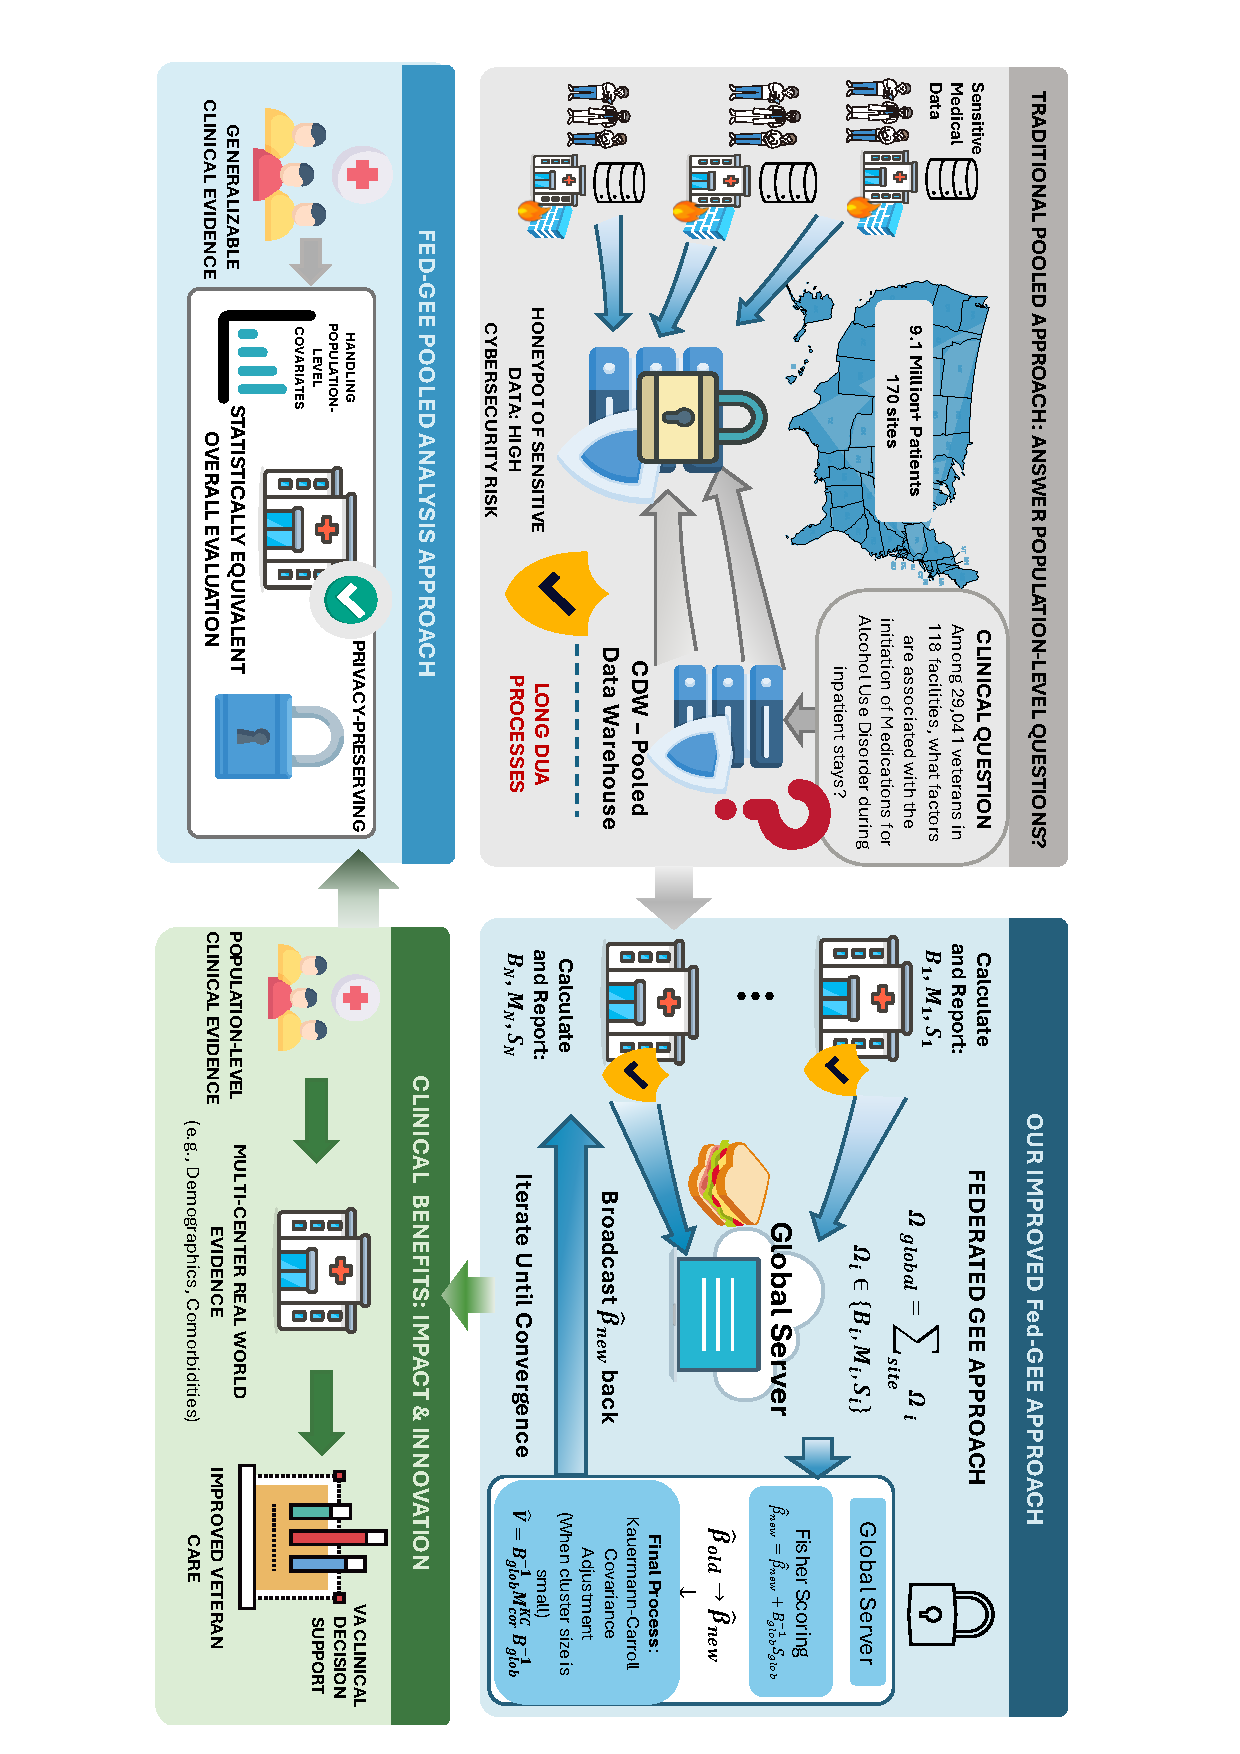
\includegraphics[width=0.95\textwidth]{Figure 1_V2.pdf}
    \caption{\textbf{Schematic of the Fed-GEE Privacy-Preserving Architecture} 
     While traditional pooled methods risk exposing sensitive medical data, the decentralized Fed-GEE framework shares only local summary statistics Bread ($\boldsymbol{B_i}$), Score ($\boldsymbol{S_i}$), and Meat ($\boldsymbol{M_i}$) matrices for global Fisher Scoring optimization and KC small sample adjustments. This approach ensures statistical equivalence and data privacy, leveraging population-level evidence to enhance clinical decision making and Veteran care.
    }
\label{fig:Figure1}
\end{figure}

%\feier{In Biometrics paper, $\widetilde{\mathbf{S}}_i = (I-H_{ii})^{-1}\mathbf{S}_i$, should we use $-1/2$ or $-1$? Since $-1/2$ version works in simulation section, should we briefly introduce why we decide to use $-1/2$? also need to cite \citep{HC2}, which offer theoretical support if we decide to use $-1/2$ version. }
%\soumik{good catch, have fixed. was confused with another reference.}

\emph{Inference:} Wald-type inference is conducted using a standard normal approximation, with the option to utilize a $t$-distribution to better account for finite-sample variability when the number of clusters is small. 

\vspace{0.5cm}
\textbf{3. Theoretical Properties}

\noindent In this section we demonstrate that the distributed parameter estimation is both consistent and asymptotically normal. We focus our asymptotic regime on the number of independent clusters (hospitals or sites) approaching infinity ($K \to \infty$), which aligns with our site-level variance estimation strategy. Let $\boldsymbol{\beta}_0$ denote the true population parameter vector that lies in the interior of a compact parameter space $\boldsymbol{\Theta} \subset \mathbb{R}^p$. Note that, in the interest of saving space, we only state the relevant technical results in the  manuscript and present detailed proofs in supplements B and C.

\emph{Regularity conditions:} We assume the following standard regularity conditions hold.
\begin{assumption}[Mean specification]\label{ass:1}
The marginal mean is correctly specified, such that $E(Y_{ijk} \mid \mathbf{X}_{ijk}) = \mu_{ijk}$, and is correctly linked to the covariates via $g(\mu_{ijk}) = \mathbf{X}_{ijk}^T \boldsymbol{\beta}_0$.
\end{assumption}
\begin{assumption}[Bounded cluster sizes]\label{ass:2}
The total number of observations at each site $i$, denoted as $N_i = \sum_{j=1}^{n_i} m_{ij}$, is uniformly bounded such that $\max_i N_i \le C < \infty$ for some constant $C$.
\end{assumption}
\begin{assumption}[Bounded covariates]\label{ass:3}
The $p$-dimensional covariate vectors $\mathbf{X}_{ijk}$ are uniformly bounded in probability. Formally, for any $\epsilon > 0$, there exists a finite constant $M > 0$ such that $\mathcal{P}\left(\left| \left|\mathbf{X}_{ijk}\right| \right| > M\right) < \epsilon$ for all sites $i$, patients $j$, and visits $k$.
\end{assumption}
\begin{assumption}[Positive definiteness]\label{ass:4}
As $K \to \infty$, there exist deterministic, finite, and positive definite matrices $\mathcal{B}(\boldsymbol{\beta}_0)$ and $\mathcal{M}(\boldsymbol{\beta}_0)$ such that $K^{-1} \sum_{i=1}^K \mathbf{B}_i(\boldsymbol{\beta}_0) \xrightarrow{p} \mathcal{B}(\boldsymbol{\beta}_0)$ and $K^{-1} \sum_{i=1}^K E\left[\mathbf{S}_i(\boldsymbol{\beta}_0) \mathbf{S}_i(\boldsymbol{\beta}_0)^T \right] \xrightarrow{p} \mathcal{M}(\boldsymbol{\beta}_0)$.
\end{assumption}

In Theorem \ref{thm:equivalence}, we establish that the distributed architecture of Fed-GEE does not alter the finite-sample root of the centralized, or pooled GEE. Next, in Theorem \ref{thm:asymptotics}, we establish technical guarantees on the large-sample behavior of Fed-GEE.

\begin{theorem}[Algebraic Equivalence]
\label{thm:equivalence}
Given the same starting value $\boldsymbol{\beta}^{(0)}$ and step size, the sequence of parameter updates $\{\boldsymbol{\beta}^{(m)}_{fed}\}$ generated by the Fed-GEE algorithm is algebraically identical to the sequence $\{\boldsymbol{\beta}^{(m)}_{cen}\}$ generated by the centralized GEE algorithm applied to the pooled dataset. Consequently, upon convergence, $\hat{\boldsymbol{\beta}}_{fed} = \hat{\boldsymbol{\beta}}_{cen}$.
\end{theorem}

\begin{theorem}[Asymptotic Properties of Fed-GEE]
\label{thm:asymptotics}
Under assumptions \autoref{ass:1}-\autoref{ass:4}, as the number of sites $K \to \infty$, the Fed-GEE estimator, $\hat{\boldsymbol{\beta}}_{fed} \xrightarrow{p} \boldsymbol{\beta}_0$, and it is asymptotically multivariate normal: $\sqrt{K}(\hat{\boldsymbol{\beta}}_{fed} - \boldsymbol{\beta}_0) \xrightarrow{d} \mathcal{N}\left(\mathbf{0}, \mathcal{B}^{-1}(\boldsymbol{\beta}_0) \mathcal{M}(\boldsymbol{\beta}_0) \mathcal{B}^{-1}(\boldsymbol{\beta}_0)\right)$. Furthermore, the finite-sample Kauermann-Carroll correction is asymptotically negligible, meaning $\mathbf{M}_{global}^{KC} \xrightarrow{p} \mathbf{M}_{global}$ as $K \to \infty$.
\end{theorem}
\textbf{4. Simulation Studies}

\noindent To evaluate the finite-sample properties of the Fed-GEE framework, we conducted a comprehensive simulation study. The primary objectives were to demonstrate the exact mathematical equivalence between Fed-GEE and centralized GEE, evaluate its robustness against naive meta-analytical estimates under complex clustering, and assess the performance of its variance estimators across varying network topologies. Comprehensive graphical and tabular results are provided in Figures \ref{fig:fig2}, \ref{fig:fig3}, and Table \ref{tab:sim-coverage}.

\emph{Data generating process:} We simulated a multi-center hierarchical data structure reflecting the VHA system: longitudinal visits ($k = 1, \dots, m_{ij}$) nested within patients ($j = 1, \dots, n_i$), who are nested within isolated hospitals ($i = 1, \dots, K$). The true marginal probability of the binary outcome, $p_{ijk}$, was specified via a logistic model: $$\text{logit}(p_{ijk}) = \beta_0 + \beta_X X_{ijk} + \beta_{\text{teach}} \text{Teaching}_i,$$  where $X_{ijk} \sim \mathcal{N}(0, 1)$ is a continuous observation-level covariate, $\text{Teaching}_i \in \{0, 1\}$ is a site-level indicator denoting whether the $i$-th hospital is a teaching facility (1) or a non-teaching facility (0). To induce the desired multi-level correlation structure while strictly preserving the specified marginal probabilities, we utilized a latent Gaussian copula approach \citep{peter2007correlated}. A latent variable was generated as $Z_{ijk} = \sqrt{\rho_H} U_i + \sqrt{\rho_P - \rho_H} W_{ij} + \sqrt{1 - \rho_P} \epsilon_{ijk}$, where $U_i, W_{ij}$, and $\epsilon_{ijk}$ are mutually independent standard normal variates. The parameters $\rho_H$ and $\rho_P$ control the intra-class correlation at the hospital and patient levels, respectively. The binary outcome was generated by thresholding the latent variable: $Y_{ijk} = I(Z_{ijk} < \Phi^{-1}(p_{ijk}))$, where $\Phi^{-1}$ is the standard normal quantile function and $I$ is the indicator variable.

Simulations were run across a parameter grid spanning $K \in [5, 100]$ hospitals, with $n_i \sim \text{Uniform}(10, 30)$ and $m_{ij} \sim \text{Uniform}(2, 6)$. We evaluated scenarios with a common outcome ($\beta_0 = -1$) and a rare outcome ($\beta_0 = -3$). We fixed $\beta_X = 1$ and $\beta_{\text{teach}} = 0.5$. The between-hospital correlation ($\rho_H$) varied from $0$ to $0.20$, and the total patient-level correlation ($\rho_P$) varied from $0.225$ to $0.40$. Each unique parameter combination was replicated 200 times. 

\emph{Simulation Results:} The performance of the evaluated methods was assessed using absolute bias, empirical standard deviation (SD), mean estimated standard error (SE), the SE/SD ratio, and 95\% coverage probability.
\begin{figure}[htbp]
    \centering
    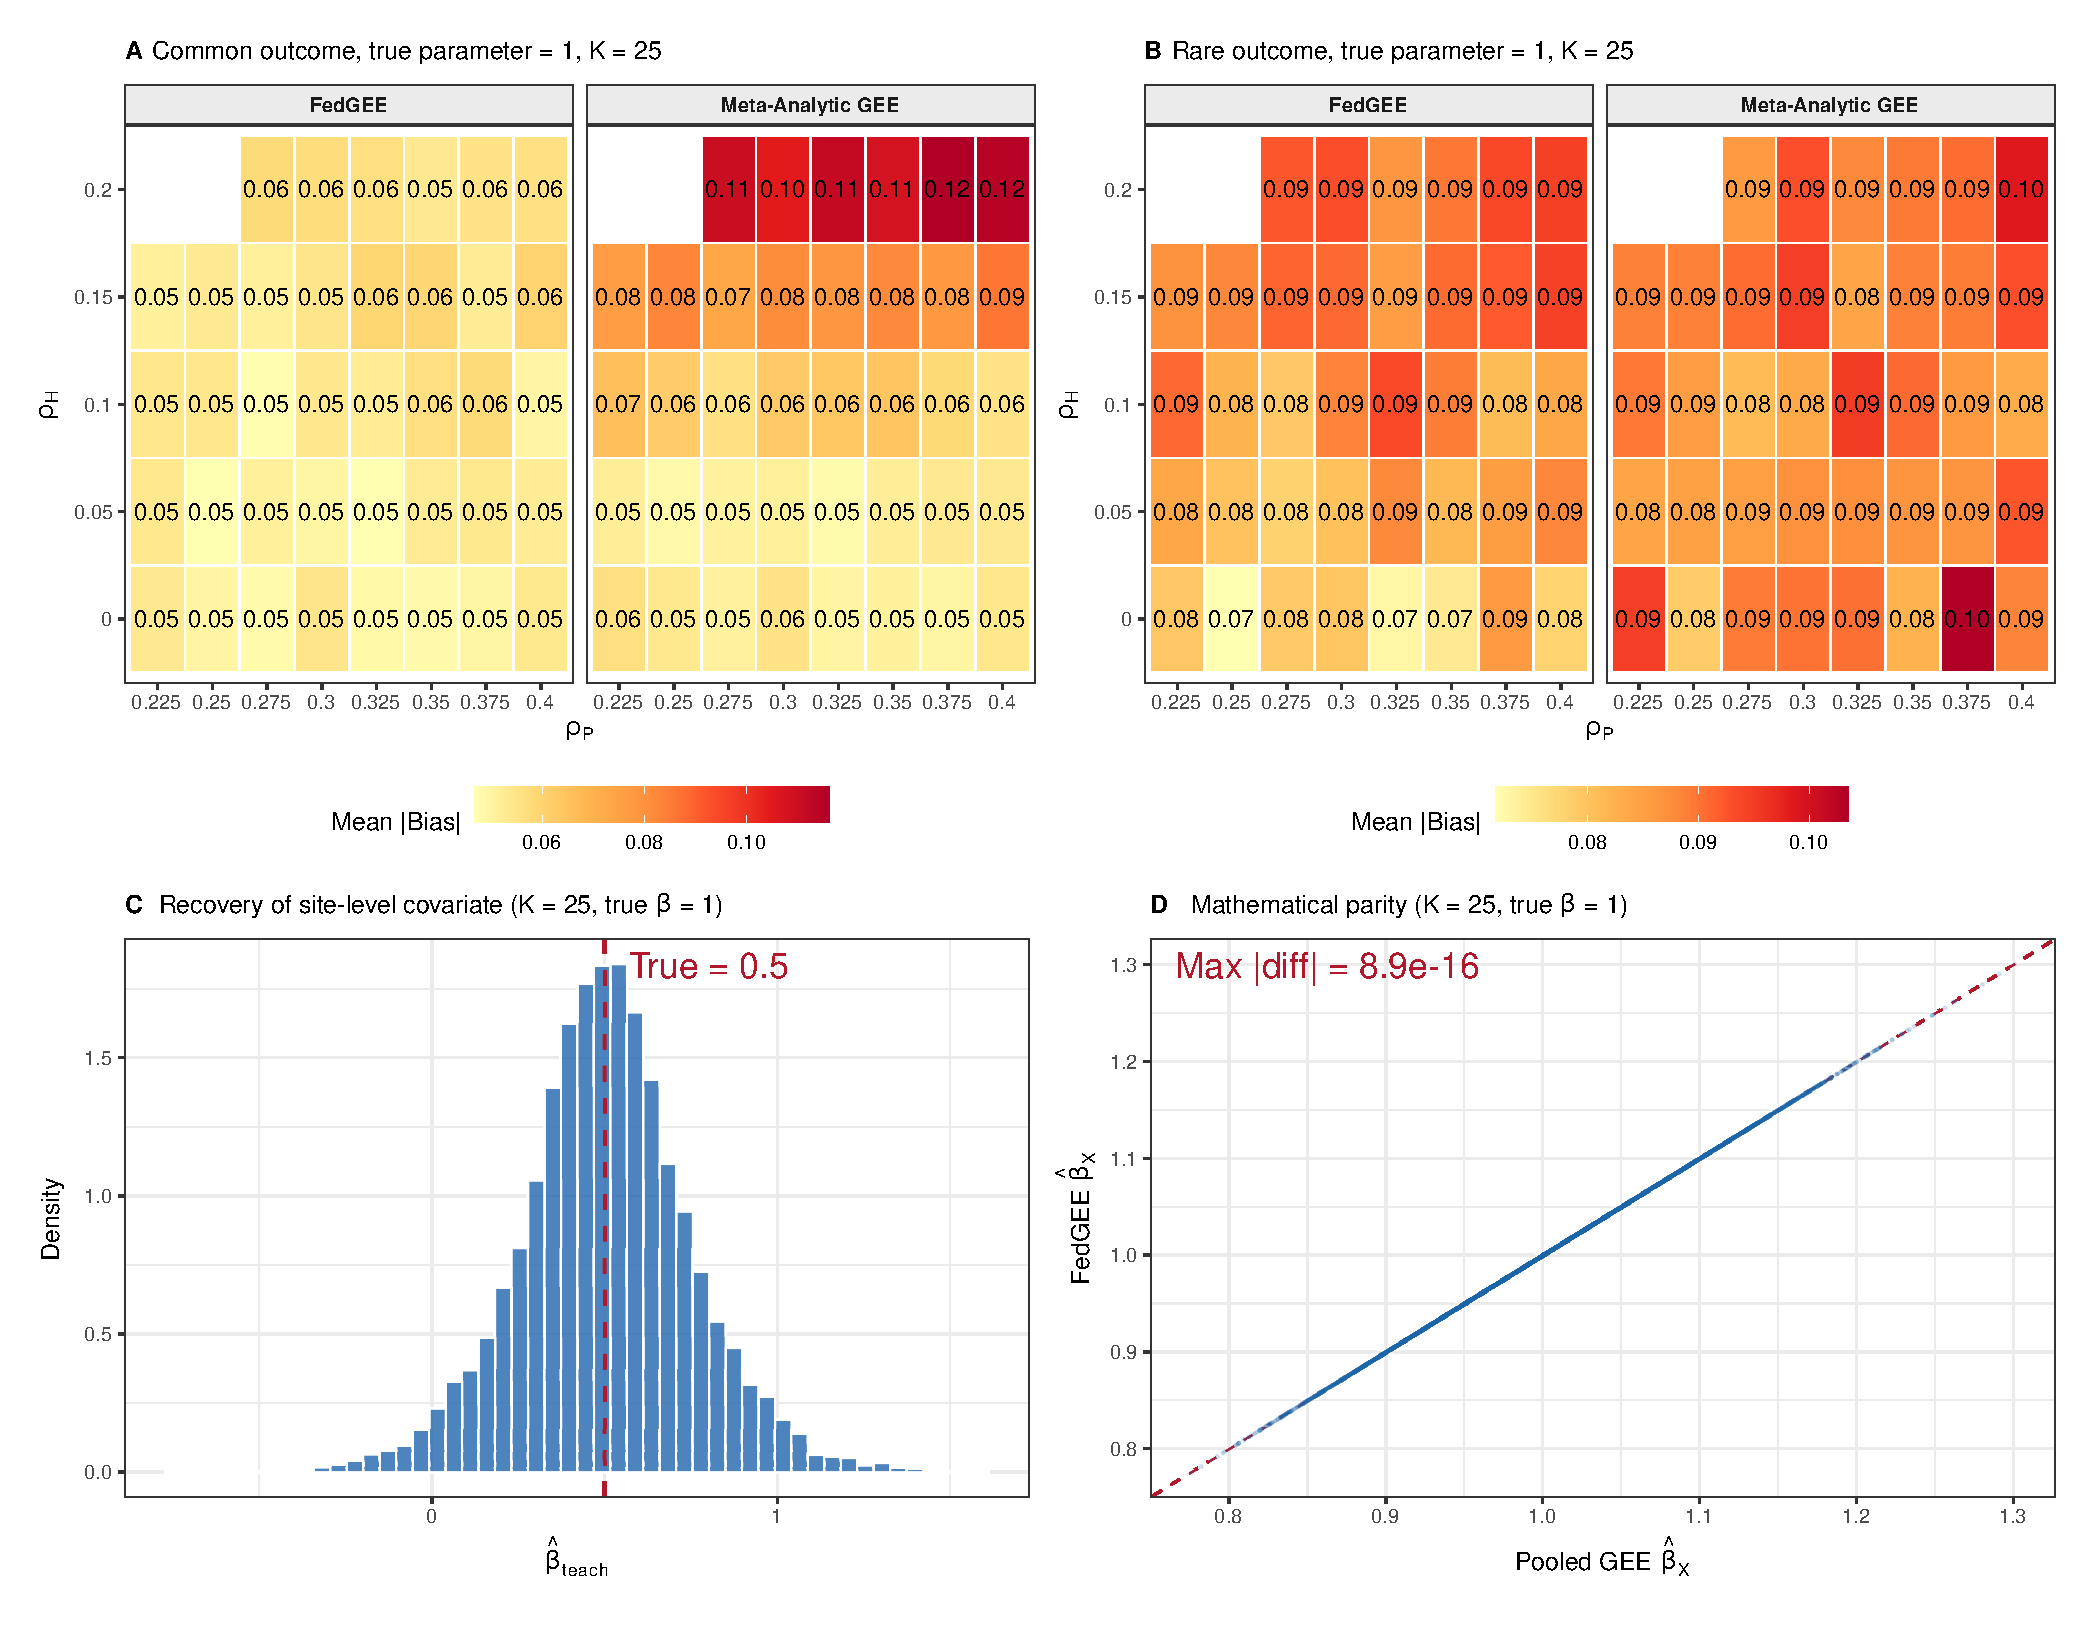
\includegraphics[angle=90, width=\textwidth]{fig2.eps}
    \caption{\textbf{Point Estimation and Bias in Federated vs.\ Traditional Networks} ($K = 25$, $\beta_0 = -1$ unless noted). \textbf{(A)}~Mean absolute bias of Fed-GEE vs.\ Meta-Analytic GEE across the $\rho_H \times \rho_P$ grid under a common outcome. \textbf{(B)}~Same comparison under a rare outcome ($\beta_0 = -3$). \textbf{(C)}~Sampling distribution of the site-level covariate estimate $\hat{\beta}_{\text{teach}}$ from Fed-GEE, recovered purely from between-site variation. \textbf{(D)}~Fed-GEE vs.\ centralized pooled GEE estimates with maximum absolute difference annotated.}
\label{fig:fig2}
\end{figure}
Figure \ref{fig:fig2} examines bias performance of Fed-GEE. As illustrated in the common outcome heatmap (\emph{Figure 2A}), the meta-analytic GEE exhibited substantial bias that increased proportionally with the hospital-level correlation ($\rho_H$). Under the rare outcome scenario (\emph{Figure 2B}), the local meta-analytic models frequently failed to converge due to sparse local event counts, rendering the standard meta-analytic method fundamentally unviable for modeling rare events in distributed networks. Furthermore, by estimating site-constant covariates entirely through between-site variation during the server update, Fed-GEE unbiasedly recovered the effect of the teaching hospital indicator ($\beta_{\text{teach}}$) (see \emph{Figure 2C}). Finally, Fed-GEE achieved exact mathematical parity with pooled GEE estimate (see \emph{Figure 2D}). 
\begin{table}[htbp]
  \caption{Performance of Variance Estimators by Number of Network Sites ($K$). Coverage probabilities and SE/SD ratios are shown for varying sandwich architectures and small-sample corrections within the Fed-GEE framework. Target coverage is $\boldsymbol{0.950}$; target SE/SD ratio is $\boldsymbol{1.00}$. Values reflect simulations where $\rho_H > 0$. Patient-level sandwich assumes independence between patients. The SE/SD ratio is identical for the site-level $z$ and $t$ rows (same standard error estimate; only the critical value differs) and is reported once. KC = Kauermann-Carroll correction.}
  \label{tab:sim-coverage}
  \resizebox{\textwidth}{!}{%
  \begin{tabular}{l cc cc c cc}
    \toprule
    & \multicolumn{2}{c}{Patient Sandwich ($z$)}
    & \multicolumn{2}{c}{Site Sandwich ($z$)}
    & \multicolumn{1}{c}{Site Sandwich ($t$)}
    & \multicolumn{2}{c}{Site + KC ($t$)} \\
    \cmidrule(lr){2-3} \cmidrule(lr){4-5} \cmidrule(lr){6-6} \cmidrule(lr){7-8}
    $K$ & Coverage & SE/SD & Coverage & SE/SD & Coverage & Coverage & SE/SD \\
    \midrule
    5   & 0.929 & 0.88 & 0.816 & 0.73 & 0.940 & 0.959 & 0.84 \\
    10  & 0.932 & 0.90 & 0.885 & 0.84 & 0.929 & 0.941 & 0.89 \\
    15  & 0.932 & 0.90 & 0.906 & 0.88 & 0.932 & 0.941 & 0.92 \\
    25  & 0.936 & 0.91 & 0.926 & 0.92 & 0.939 & 0.946 & 0.94 \\
    50  & 0.934 & 0.91 & 0.937 & 0.94 & 0.943 & 0.946 & 0.95 \\
    100 & 0.935 & 0.92 & 0.944 & 0.96 & 0.947 & 0.948 & 0.96 \\
    \bottomrule
  \end{tabular}}&
\end{table}
Table \ref{tab:sim-coverage} evaluates the performance of the variance estimators. As expected, standard patient-level and site-level sandwich estimators suffered from severe under-coverage at finite cluster sizes. Applying the KC correction with a $t$-distribution substantially mitigated this downward bias. However, the correction is not absolute; for highly restricted federated consortia ($K\leq15$), the KC-corrected estimator still exhibits nominal under-coverage (ranging from $0.84$ to $0.94$) and underestimates the empirical standard deviation. Researchers should exercise caution when applying this framework to networks with fewer than $25$ independent sites. 


\vspace{0.5cm}
\textbf{5. Application}

\noindent To demonstrate the practical utility of the FedGEE framework, we applied the method to a national cohort of $n = 29,041$ Veterans diagnosed with AUD across $K = 118$ facilities in the Veterans Health Administration (VHA). We modeled post-hospitalization initiation of MAUD against demographics (age, sex, race/ethnicity, rurality, and Area Deprivation Index (ADI)), substance use history (prior-year MAUD, AUDIT-C, opioid use disorder), medical complexity (VA Care Assessment Need (CAN) score, frailty category, and ICU care), and hospitalization factors (specialty, disposition, addiction consults); see Supplementary Table 1. Fitting a facility-clustered logistic GEE with an exchangeable working correlation, we evaluated Fed-GEE against a centralized pooled GEE. Fed-GEE achieved exact point-estimate parity with the centralized model (Figure~\ref{fig:fig2}), yielding numerically identical adjusted odds ratios (aORs). 
\begin{figure}[htbp]
    \centering
    \includegraphics[height=0.9\textheight]{fig3.eps}
    \caption{Forest plot showing adjusted odds ratios for MAUD initiation following inpatient discharge ($N=29,041$; $K=118$ VHA facilities). Centralized pooled GEE (blue) and privacy-preserving Fed-GEE with KC correction (orange). Point estimates are numerically identical; confidence intervals for Fed-GEE are wider due to the small-sample correction and 
$t$-based inference.}
    \label{fig:fig3}
\end{figure}
Clinically, prior-year MAUD use (aOR$=2.04, 95\%$ Confidence Interval (CI): $1.87-2.22$) and discharge from a psychiatry specialty (aOR$=1.72, 95\%$ CI: $1.34-2.20$) strongly predicted MAUD initiation. However, the most critical difference between the models emerged in the confidence intervals. Standard sandwich standard errors (SEs) used in centralized GEE treat the massive number of patients as the effective sample size, severely understating uncertainty when the number of independent clusters ($K=118$) is the statistically relevant quantity. By utilizing KC-corrected SEs and $t$-based inference, Fed-GEE provided calibrated wider confidence intervals. Consequently, several covariates that appeared statistically significant under the naive pooled GEE lost their nominal significance ($p > 0.05$) under the corrected federated framework. Specifically, while the uncorrected pooled GEE suggested that female sex, rural residency, high area deprivation (ADI $76-100$), higher medical complexity (VA CAN quintiles $3-5$), ICU stays, and both clinical and non-clinical addiction consults were all significantly associated with MAUD initiation, none of these factors remained significant after applying the KC small-sample cluster correction. This discrepancy underscores the severe practical consequences of ignoring the cluster-level effective sample size; failing to adjust for the network topology would have led to spurious clinical and policy conclusions regarding healthcare disparities and care pathways across the VHA.

\vspace{0.5cm}
\textbf{6. Discussion and concluding remarks}
\noindent 


Fed-GEE is most useful when the goal is a population-averaged treatment effect estimated from multi-site data that cannot, or should not, be centralized. The algebraic equivalence guarantee ensures no statistical cost to federation: the point estimates match what a pooled analysis would yield. When the question is instead facility-specific or conditional on unobserved heterogeneity, a mixed-effects approach is recommended \citep{luo2022dlmm}.

Three limitations of the current framework point to natural extensions. First, we fixed the working correlation to exchangeable throughout. This is safe for consistency but may sacrifice efficiency. A federated analogue of the Quasilikelihood Information Criterion (QIC) \citep{pan2001akaike}, decomposing the quasi-likelihood across sites without sharing residuals, would allow data-driven structure selection within the protocol. Second, the current protocol relies on a trusted central server to aggregate site contributions and broadcast parameters. Replacing this  with a decentralized variant \citep{gu2024statistical}, where sites converge via peer-to-peer consensus without a central aggregator, would eliminate the single point of failure, reduce communication exposure, and relax the trust assumptions of the network. Third, while our algorithm successfully incorporated the Kauermann-Carroll (KC) correction to mitigate finite-sample under-coverage, the KC estimator primarily targets bias in the covariance matrix itself. Future work will expand the federated architecture to incorporate the Mancl-DeRouen (MD) \citep{mancl2001covariance} small-sample correction, which may provide superior Type I error control for hypothesis testing in federated networks with fewer sites. 
%Finally, we note that a formal evaluation of differential privacy \citep{dwork2006calibrating} would strengthen the privacy guarantees of Fed-GEE from heuristic to mathematically provable, and would be another avenue of future research.

\label{lastpage}


\bibliographystyle{biom}
\bibliography{02_bibliography}


\clearpage
\FloatBarrier





\end{document}